\documentclass[11pt]{article}
\usepackage[margin=1in]{geometry}
\usepackage{amsmath,amssymb,graphicx,booktabs,longtable}
\title{q-ridge: certifying the empirical quadrature of a Burgers correction ladder\\
on the states the reduced model actually reaches}
\date{2026-09-16}
\begin{document}\maketitle
\section{q-ridge -- the regression is the quadrature rule; certifying it on reachable states removes almost all of it, but not the top rung within the constructible $m \le 2048$}
Final numbers. Three cluster jobs on the frozen Burgers checkpoint 18f0266ae6f0… at 256 intervals, on the six opened development cases, under the budget-600 block-damped variable-projection contract inherited from b-ladder-top. The pre-registered design and its amendment §A3, which re-scoped the lane after the q-diag lane reported, are in [../DESIGN.md](../DESIGN.md).

\begin{table}[htbp]\centering\small
\begin{tabular}{llllllll}\hline
job & attempt & question & job id & GPU & source commit & elapsed (s) & failed gates \\ \hline
1 & qrg101 & R1 & 3757235 & NVIDIA A100 80GB PCIe & 5fc6099127d4 & 5389.4 & none \\
2 & qrg201 & R2 & 3757237 & NVIDIA A100 80GB PCIe & 5fc6099127d4 & 6834.0 & none \\
3 & qrg304 & EQCERT & 3768168 & NVIDIA A100 80GB PCIe & 467a4670f179 & 10502.3 & none \\
\hline\end{tabular}
\end{table}
\subsection{Where the regression is, measured before anything was submitted}
Recomputed from the retained cclad01 fields (job 3734098, archive SHA256 4c6fd589688a253f…), worst over the six cases, against that job's own converged full-order solve. The q-diag lane reached the same conclusion independently and across four jobs.

\begin{table}[htbp]\centering\small
\begin{tabular}{lllllll}\hline
configuration & $q=0$ & $q=16$ & $q=32$ & $q=64$ & $q=128$ & monotone in $q$? \\ \hline
m4 dense & 1.8890 & 1.3984 & 1.2336 & 1.0843 & 0.8930 & yes \\
M=256 dense & 1.2710 & 1.2305 & 1.1869 & 1.1255 & 1.0418 & yes \\
M=256 EQ & 1.3113 & 1.4956 & 1.5231 & 1.5557 & 1.6141 & no \\
m4 EQ & 1.9002 & 2.9937 & -- & -- & -- & no \\
\hline\end{tabular}
\end{table}
The dense and the EQ arms at $M=256$ solve the **identical** $M$ test equations against the **identical** $K+q$ unknowns; the only difference is that the advection integral is replaced by an $m$-point rule. The dense ladder is monotone and the EQ ladder is not.

\subsection{EQ rule certification -- the primary}
**Verdict: no.** The incumbent rule's ladder is non-monotone on the evolved metric; every rung of the rebuilt ladder certified at the primary bar: no; the top rung certified: no. No $m$ in the declared grid reaches the bar at the top rung; a log-log extrapolation of $\rho_{\max}$ against $m$ puts the crossing at $m \approx 2522$ (slope -1.772).

\subsubsection{The reachable-state population}
\begin{table}[htbp]\centering\small
\begin{tabular}{llllll}\hline
$q$ & $M$ & iterates per step & fit states available & certification states available & collection (s) \\ \hline
0 & 64 & 13 & 15600 & 5200 & 23.8 \\
16 & 128 & 13 & 15600 & 5200 & 27.1 \\
32 & 192 & 13 & 15600 & 5200 & 32.8 \\
64 & 320 & 13 & 15600 & 5200 & 43.6 \\
128 & 576 & 13 & 15600 & 5200 & 66.5 \\
256 & 1088 & 13 & 15600 & 5200 & 132.7 \\
\hline\end{tabular}
\end{table}
\subsubsection{Certification: every rule, its NNLS fit and its held-out $\rho$}
The bar is $\rho^\star = 0.116$, declared in DESIGN.md §A3.4 before the job ran, from q-diag's measurement of the $q=0$ incumbent rule. **A rule is never certified by its NNLS relative fit**, which is reported here precisely so the anti-correlation can be seen again on new rules.

\begin{table}[htbp]\centering\small
\begin{tabular}{llllllllllll}\hline
$q$ & population & $m$ target & $m$ achieved & $m/M$ & NNLS relative fit & $\rho_{\max}$ & $\rho_{95}$ & $\rho_{\rm med}$ & certified & truncated & fit (s) \\ \hline
0 & reachable & 1024 & 1024 & 16.00 & 4.58e-05 & 0.0153 & 0.0088 & 0.0005 & yes & no & 71.5 \\
0 & reachable & 2048 & 1521 & 23.77 & 7.83e-06 & 0.0261 & 0.0083 & 0.0002 & yes & no & 116.7 \\
0 & static & 256 & 256 & 4.00 & 6.85e-03 & 0.2407 & 0.2073 & 0.0153 & no & no & 6.0 \\
16 & reachable & 1024 & 1024 & 8.00 & 1.90e-04 & 0.0935 & 0.0273 & 0.0007 & yes & no & 146.5 \\
16 & reachable & 2048 & 2048 & 16.00 & 1.92e-05 & 0.0452 & 0.0041 & 0.0002 & yes & no & 641.6 \\
16 & static & 512 & 512 & 4.00 & 1.54e-03 & 0.1279 & 0.0523 & 0.0024 & no & no & 48.0 \\
32 & reachable & 1024 & 1024 & 5.33 & 2.89e-04 & 0.0533 & 0.0226 & 0.0014 & yes & no & 154.7 \\
32 & reachable & 2048 & 2048 & 10.67 & 2.66e-05 & 0.0668 & 0.0120 & 0.0002 & yes & no & 650.7 \\
32 & static & 768 & 768 & 4.00 & 6.27e-04 & 0.1482 & 0.0214 & 0.0015 & no & no & 99.6 \\
64 & reachable & 1024 & 1024 & 3.20 & 7.12e-04 & 0.0531 & 0.0230 & 0.0027 & yes & no & 159.9 \\
64 & reachable & 2048 & 2048 & 6.40 & 7.54e-05 & 0.1120 & 0.0172 & 0.0010 & yes & no & 656.1 \\
64 & static & 1280 & 1280 & 4.00 & 2.43e-04 & 0.1439 & 0.0235 & 0.0015 & no & no & 275.3 \\
128 & reachable & 1024 & 1024 & 1.78 & 1.62e-03 & 0.2786 & 0.2246 & 0.0177 & no & no & 238.2 \\
128 & reachable & 2048 & 2048 & 3.56 & 1.04e-04 & 0.1908 & 0.0518 & 0.0019 & no & no & 781.1 \\
128 & static & 2048 & 2048 & 3.56 & 7.16e-05 & 0.2194 & 0.0677 & 0.0016 & no & no & 840.8 \\
256 & reachable & 1024 & 1024 & 0.94 & 4.01e-02 & 0.5731 & 0.5370 & 0.1855 & no & no & 100.1 \\
256 & reachable & 2048 & 2048 & 1.88 & 3.08e-04 & 0.1678 & 0.0957 & 0.0099 & no & no & 962.1 \\
256 & static & 2048 & 2048 & 1.88 & 1.49e-04 & 0.4621 & 0.4275 & 0.0585 & no & no & 1485.1 \\
\hline\end{tabular}
\end{table}
\subsubsection{The rule chosen at each rung}
\begin{table}[htbp]\centering\small
\begin{tabular}{lllllll}\hline
$q$ & $M$ & chosen $m$ & basis & $\rho_{\max}$ & $\rho_{95}$ & NNLS relative fit \\ \hline
0 & 64 & 1024 & primary & 0.0153 & 0.0088 & 4.58e-05 \\
16 & 128 & 1024 & primary & 0.0935 & 0.0273 & 1.90e-04 \\
32 & 192 & 1024 & primary & 0.0533 & 0.0226 & 2.89e-04 \\
64 & 320 & 1024 & primary & 0.0531 & 0.0230 & 7.12e-04 \\
128 & 576 & 2048 & secondary & 0.1908 & 0.0518 & 1.04e-04 \\
256 & 1088 & 2048 & secondary & 0.1678 & 0.0957 & 3.08e-04 \\
\hline\end{tabular}
\end{table}
\subsubsection{The dense ladder this is measured against}
Read-only from the q-trajdirs lane, job 3757505 (qtd02) on NVIDIA A100-PCIE-40GB: the same six cases, the same old direction rule, the same budget-600 contract, exact quadrature, $M = 4(K+q)$. It is the ladder the empirical rule has to reproduce.

\begin{table}[htbp]\centering\small
\begin{tabular}{llllll}\hline
$q$ & $M$ & worst evolved \% & worst all-times \% & median GPU ms & converged \\ \hline
0 & 64 & 1.8890 & 2.5629 & 333.2 & yes \\
16 & 128 & 1.3985 & 2.4806 & 417.9 & yes \\
32 & 192 & 1.2336 & 2.3534 & 496.9 & yes \\
64 & 320 & 1.0843 & 2.1489 & 701.7 & yes \\
128 & 576 & 0.8930 & 1.8116 & 1330.4 & yes \\
256 & 1088 & 0.5194 & 0.9053 & 4354.9 & yes \\
\hline\end{tabular}
\end{table}
Monotone on the evolved metric: **yes**.

\subsubsection{The rebuilt ladder}
**EQ, cheapest certified rule per rung** -- monotone on evolved times: **no**; monotone on all times: yes; every rung converged: yes; cost within 2x of the old rule: yes; all-times not raised: yes; **passes: no**.

\begin{table}[htbp]\centering\small
\begin{tabular}{lllllllllll}\hline
$q$ & $M$ & $m$ & $\rho_{\max}$ & certified & worst evolved \% & worst all-times \% & $t=0$ compression \% & median GPU ms & converged & cost vs old rule \\ \hline
0 & 64 & 1024 & 0.0153 & yes & 1.8891 & 2.5629 & 2.5629 & 57.4 & yes & 1.129x \\
16 & 128 & 1024 & 0.0935 & yes & 1.4270 & 2.4806 & 2.4806 & 79.2 & yes & 1.106x \\
32 & 192 & 1024 & 0.0533 & yes & 1.2493 & 2.3534 & 2.3534 & 96.0 & yes & 1.063x \\
64 & 320 & 1024 & 0.0531 & yes & 1.2275 & 2.1489 & 2.1489 & 118.6 & yes & 0.957x \\
128 & 576 & 2048 & 0.1908 & no & 0.8925 & 1.8116 & 1.8116 & 246.8 & yes & 1.006x \\
256 & 1088 & 2048 & 0.1678 & no & 1.0361 & 1.0361 & 0.9053 & 699.3 & yes & 1.015x \\
\hline\end{tabular}
\end{table}
**EQ, incumbent static-population rule** -- monotone on evolved times: **no**; monotone on all times: no; every rung converged: yes.

\begin{table}[htbp]\centering\small
\begin{tabular}{llllllllll}\hline
$q$ & $M$ & $m$ & $\rho_{\max}$ & certified & worst evolved \% & worst all-times \% & $t=0$ compression \% & median GPU ms & converged \\ \hline
0 & 64 & 256 & 0.2407 & no & 3.4166 & 3.4166 & 2.5629 & 50.8 & yes \\
16 & 128 & 512 & 0.1279 & no & 2.1427 & 2.4806 & 2.4806 & 71.6 & yes \\
32 & 192 & 768 & 0.1482 & no & 1.5026 & 2.3534 & 2.3534 & 90.4 & yes \\
64 & 320 & 1280 & 0.1439 & no & 1.1454 & 2.1489 & 2.1489 & 123.9 & yes \\
128 & 576 & 2048 & 0.2194 & no & 0.8928 & 1.8116 & 1.8116 & 245.4 & yes \\
256 & 1088 & 2048 & 0.4621 & no & 6.0676 & 6.0676 & 0.9053 & 688.6 & yes \\
\hline\end{tabular}
\end{table}
**dense (exact) quadrature** -- monotone on evolved times: **yes**; monotone on all times: yes; every rung converged: yes.

\begin{table}[htbp]\centering\small
\begin{tabular}{llllllllll}\hline
$q$ & $M$ & $m$ & $\rho_{\max}$ & certified & worst evolved \% & worst all-times \% & $t=0$ compression \% & median GPU ms & converged \\ \hline
0 & 64 & -- & -- & -- & 1.8890 & 2.5629 & 2.5629 & 281.9 & yes \\
64 & 320 & -- & -- & -- & 1.0843 & 2.1489 & 2.1489 & 620.4 & yes \\
256 & 1088 & -- & -- & -- & 0.5194 & 0.9053 & 0.9053 & 3945.3 & yes \\
\hline\end{tabular}
\end{table}
\subsection{R1 (control) -- the field-metric ridge}
\subsubsection{Dense (exact) quadrature}
**$\lambda_{rel} = 0$** -- monotone in $q$ on evolved times: **yes**; every rung converged: yes; cost within 1.5x of the incumbent: yes; all-times metric not raised: yes; **passes: yes**.

\begin{table}[htbp]\centering\small
\begin{tabular}{llllllllll}\hline
$q$ & $M$ & $m$ & worst evolved \% & worst all-times \% & $t=0$ compression \% & median GPU ms & cost vs incumbent & converged & EQ rule valid \\ \hline
0 & 64 & -- & 1.8890 & 2.5629 & 2.5629 & 295.2 & 1.000x & yes & -- \\
16 & 128 & -- & 1.3985 & 2.4806 & 2.4806 & 368.0 & 1.000x & yes & -- \\
64 & 320 & -- & 1.0843 & 2.1489 & 2.1489 & 627.2 & 1.000x & yes & -- \\
256 & 1088 & -- & 0.5194 & 0.9053 & 0.9053 & 3911.9 & 1.000x & yes & -- \\
\hline\end{tabular}
\end{table}
**$\lambda_{rel} = 0.0001$** -- monotone in $q$ on evolved times: **yes**; every rung converged: yes; cost within 1.5x of the incumbent: yes; all-times metric not raised: yes; **passes: yes**.

\begin{table}[htbp]\centering\small
\begin{tabular}{llllllllll}\hline
$q$ & $M$ & $m$ & worst evolved \% & worst all-times \% & $t=0$ compression \% & median GPU ms & cost vs incumbent & converged & EQ rule valid \\ \hline
0 & 64 & -- & 1.8890 & 2.5629 & 2.5629 & 295.2 & 1.000x & yes & -- \\
16 & 128 & -- & 1.3983 & 2.4806 & 2.4806 & 368.7 & 1.002x & yes & -- \\
64 & 320 & -- & 1.0842 & 2.1489 & 2.1489 & 625.3 & 0.997x & yes & -- \\
256 & 1088 & -- & 0.5127 & 0.9053 & 0.9053 & 4020.5 & 1.028x & yes & -- \\
\hline\end{tabular}
\end{table}
**$\lambda_{rel} = 0.001$** -- monotone in $q$ on evolved times: **yes**; every rung converged: yes; cost within 1.5x of the incumbent: yes; all-times metric not raised: yes; **passes: yes**.

\begin{table}[htbp]\centering\small
\begin{tabular}{llllllllll}\hline
$q$ & $M$ & $m$ & worst evolved \% & worst all-times \% & $t=0$ compression \% & median GPU ms & cost vs incumbent & converged & EQ rule valid \\ \hline
0 & 64 & -- & 1.8890 & 2.5629 & 2.5629 & 295.2 & 1.000x & yes & -- \\
16 & 128 & -- & 1.3966 & 2.4806 & 2.4806 & 369.5 & 1.004x & yes & -- \\
64 & 320 & -- & 1.0830 & 2.1489 & 2.1489 & 627.4 & 1.000x & yes & -- \\
256 & 1088 & -- & 0.4727 & 0.9053 & 0.9053 & 3737.6 & 0.955x & yes & -- \\
\hline\end{tabular}
\end{table}
**$\lambda_{rel} = 0.01$** -- monotone in $q$ on evolved times: **yes**; every rung converged: yes; cost within 1.5x of the incumbent: yes; all-times metric not raised: yes; **passes: yes**.

\begin{table}[htbp]\centering\small
\begin{tabular}{llllllllll}\hline
$q$ & $M$ & $m$ & worst evolved \% & worst all-times \% & $t=0$ compression \% & median GPU ms & cost vs incumbent & converged & EQ rule valid \\ \hline
0 & 64 & -- & 1.8890 & 2.5629 & 2.5629 & 295.2 & 1.000x & yes & -- \\
16 & 128 & -- & 1.3838 & 2.4806 & 2.4806 & 369.9 & 1.005x & yes & -- \\
64 & 320 & -- & 1.0745 & 2.1489 & 2.1489 & 629.5 & 1.004x & yes & -- \\
256 & 1088 & -- & 0.4308 & 0.9053 & 0.9053 & 3032.5 & 0.775x & yes & -- \\
\hline\end{tabular}
\end{table}
**$\lambda_{rel} = 0.1$** -- monotone in $q$ on evolved times: **yes**; every rung converged: yes; cost within 1.5x of the incumbent: yes; all-times metric not raised: yes; **passes: yes**.

\begin{table}[htbp]\centering\small
\begin{tabular}{llllllllll}\hline
$q$ & $M$ & $m$ & worst evolved \% & worst all-times \% & $t=0$ compression \% & median GPU ms & cost vs incumbent & converged & EQ rule valid \\ \hline
0 & 64 & -- & 1.8890 & 2.5629 & 2.5629 & 295.2 & 1.000x & yes & -- \\
16 & 128 & -- & 1.3750 & 2.4806 & 2.4806 & 368.6 & 1.002x & yes & -- \\
64 & 320 & -- & 1.0877 & 2.1489 & 2.1489 & 633.7 & 1.010x & yes & -- \\
256 & 1088 & -- & 0.6251 & 0.9053 & 0.9053 & 2862.1 & 0.732x & yes & -- \\
\hline\end{tabular}
\end{table}
**$\lambda_{rel} = 1$** -- monotone in $q$ on evolved times: **yes**; every rung converged: yes; cost within 1.5x of the incumbent: yes; all-times metric not raised: no; **passes: no**.

\begin{table}[htbp]\centering\small
\begin{tabular}{llllllllll}\hline
$q$ & $M$ & $m$ & worst evolved \% & worst all-times \% & $t=0$ compression \% & median GPU ms & cost vs incumbent & converged & EQ rule valid \\ \hline
0 & 64 & -- & 1.8890 & 2.5629 & 2.5629 & 295.2 & 1.000x & yes & -- \\
16 & 128 & -- & 1.4297 & 2.4806 & 2.4806 & 366.9 & 0.997x & yes & -- \\
64 & 320 & -- & 1.2140 & 2.1489 & 2.1489 & 634.2 & 1.011x & yes & -- \\
256 & 1088 & -- & 1.1011 & 1.1011 & 0.9053 & 2657.6 & 0.679x & yes & -- \\
\hline\end{tabular}
\end{table}
\subsubsection{Empirical quadrature, $m = 4M$}
**$\lambda_{rel} = 0$** -- monotone in $q$ on evolved times: **no**; every rung converged: yes; cost within 1.5x of the incumbent: yes; all-times metric not raised: yes; **passes: no**.

\begin{table}[htbp]\centering\small
\begin{tabular}{llllllllll}\hline
$q$ & $M$ & $m$ & worst evolved \% & worst all-times \% & $t=0$ compression \% & median GPU ms & cost vs incumbent & converged & EQ rule valid \\ \hline
0 & 64 & 256 & 2.0659 & 2.5629 & 2.5629 & 51.8 & 1.000x & yes & yes \\
16 & 128 & 512 & 2.1811 & 2.4806 & 2.4806 & 72.4 & 1.000x & yes & yes \\
64 & 320 & 1280 & 1.1408 & 2.1489 & 2.1489 & 127.4 & 1.000x & yes & yes \\
256 & 1088 & 2048 & 3.5204 & 3.5204 & 0.9053 & 715.4 & 1.000x & yes & yes \\
\hline\end{tabular}
\end{table}
**$\lambda_{rel} = 0.0001$** -- monotone in $q$ on evolved times: **no**; every rung converged: yes; cost within 1.5x of the incumbent: yes; all-times metric not raised: yes; **passes: no**.

\begin{table}[htbp]\centering\small
\begin{tabular}{llllllllll}\hline
$q$ & $M$ & $m$ & worst evolved \% & worst all-times \% & $t=0$ compression \% & median GPU ms & cost vs incumbent & converged & EQ rule valid \\ \hline
0 & 64 & 256 & 2.0659 & 2.5629 & 2.5629 & 51.8 & 1.000x & yes & yes \\
16 & 128 & 512 & 2.1809 & 2.4806 & 2.4806 & 73.4 & 1.015x & yes & yes \\
64 & 320 & 1280 & 1.1406 & 2.1489 & 2.1489 & 127.3 & 1.000x & yes & yes \\
256 & 1088 & 2048 & 3.5155 & 3.5155 & 0.9053 & 732.1 & 1.023x & yes & yes \\
\hline\end{tabular}
\end{table}
**$\lambda_{rel} = 0.001$** -- monotone in $q$ on evolved times: **no**; every rung converged: yes; cost within 1.5x of the incumbent: yes; all-times metric not raised: yes; **passes: no**.

\begin{table}[htbp]\centering\small
\begin{tabular}{llllllllll}\hline
$q$ & $M$ & $m$ & worst evolved \% & worst all-times \% & $t=0$ compression \% & median GPU ms & cost vs incumbent & converged & EQ rule valid \\ \hline
0 & 64 & 256 & 2.0659 & 2.5629 & 2.5629 & 51.8 & 1.000x & yes & yes \\
16 & 128 & 512 & 2.1786 & 2.4806 & 2.4806 & 74.1 & 1.024x & yes & yes \\
64 & 320 & 1280 & 1.1396 & 2.1489 & 2.1489 & 126.6 & 0.994x & yes & yes \\
256 & 1088 & 2048 & 3.4804 & 3.4804 & 0.9053 & 669.1 & 0.935x & yes & yes \\
\hline\end{tabular}
\end{table}
**$\lambda_{rel} = 0.01$** -- monotone in $q$ on evolved times: **no**; every rung converged: yes; cost within 1.5x of the incumbent: yes; all-times metric not raised: yes; **passes: no**.

\begin{table}[htbp]\centering\small
\begin{tabular}{llllllllll}\hline
$q$ & $M$ & $m$ & worst evolved \% & worst all-times \% & $t=0$ compression \% & median GPU ms & cost vs incumbent & converged & EQ rule valid \\ \hline
0 & 64 & 256 & 2.0659 & 2.5629 & 2.5629 & 51.8 & 1.000x & yes & yes \\
16 & 128 & 512 & 2.1604 & 2.4806 & 2.4806 & 73.8 & 1.020x & yes & yes \\
64 & 320 & 1280 & 1.1332 & 2.1489 & 2.1489 & 127.5 & 1.001x & yes & yes \\
256 & 1088 & 2048 & 3.2834 & 3.2834 & 0.9053 & 518.4 & 0.725x & yes & yes \\
\hline\end{tabular}
\end{table}
**$\lambda_{rel} = 0.1$** -- monotone in $q$ on evolved times: **no**; every rung converged: no; cost within 1.5x of the incumbent: yes; all-times metric not raised: yes; **passes: no**.

\begin{table}[htbp]\centering\small
\begin{tabular}{llllllllll}\hline
$q$ & $M$ & $m$ & worst evolved \% & worst all-times \% & $t=0$ compression \% & median GPU ms & cost vs incumbent & converged & EQ rule valid \\ \hline
0 & 64 & 256 & 2.0659 & 2.5629 & 2.5629 & 51.8 & 1.000x & yes & yes \\
16 & 128 & 512 & 2.1247 & 2.4806 & 2.4806 & 72.8 & 1.006x & yes & yes \\
64 & 320 & 1280 & 1.1623 & 2.1489 & 2.1489 & 132.0 & 1.036x & yes & yes \\
256 & 1088 & 2048 & 2.7294 & 2.7294 & 0.9053 & 485.4 & 0.679x & no & yes \\
\hline\end{tabular}
\end{table}
**$\lambda_{rel} = 1$** -- monotone in $q$ on evolved times: **no**; every rung converged: yes; cost within 1.5x of the incumbent: yes; all-times metric not raised: yes; **passes: no**.

\begin{table}[htbp]\centering\small
\begin{tabular}{llllllllll}\hline
$q$ & $M$ & $m$ & worst evolved \% & worst all-times \% & $t=0$ compression \% & median GPU ms & cost vs incumbent & converged & EQ rule valid \\ \hline
0 & 64 & 256 & 2.0659 & 2.5629 & 2.5629 & 51.8 & 1.000x & yes & yes \\
16 & 128 & 512 & 2.1720 & 2.4806 & 2.4806 & 73.6 & 1.017x & yes & yes \\
64 & 320 & 1280 & 1.3026 & 2.1489 & 2.1489 & 130.4 & 1.024x & yes & yes \\
256 & 1088 & 2048 & 2.5988 & 2.5988 & 0.9053 & 452.3 & 0.632x & yes & yes \\
\hline\end{tabular}
\end{table}
\subsection{R2 (control) -- more tests at fixed $q$}
\subsubsection{Dense (exact) quadrature}
**$M = 16(K+q)$** -- monotone in $q$ on evolved times: **yes**; every rung converged: yes; cost within 1.5x of the incumbent: no; all-times metric not raised: yes; **passes: no**.

\begin{table}[htbp]\centering\small
\begin{tabular}{llllllllll}\hline
$q$ & $M$ & $m$ & worst evolved \% & worst all-times \% & $t=0$ compression \% & median GPU ms & cost vs incumbent & converged & EQ rule valid \\ \hline
0 & 256 & -- & 1.2710 & 2.5629 & 2.5629 & 343.1 & 1.209x & yes & -- \\
16 & 512 & -- & 1.2204 & 2.4806 & 2.4806 & 545.2 & 1.524x & yes & -- \\
64 & 1280 & -- & 1.0588 & 2.1489 & 2.1489 & 1301.8 & 2.095x & yes & -- \\
\hline\end{tabular}
\end{table}
**$M = 4(K+q)$** -- monotone in $q$ on evolved times: **yes**; every rung converged: yes; cost within 1.5x of the incumbent: yes; all-times metric not raised: yes; **passes: yes**.

\begin{table}[htbp]\centering\small
\begin{tabular}{llllllllll}\hline
$q$ & $M$ & $m$ & worst evolved \% & worst all-times \% & $t=0$ compression \% & median GPU ms & cost vs incumbent & converged & EQ rule valid \\ \hline
0 & 64 & -- & 1.8890 & 2.5629 & 2.5629 & 283.8 & 1.000x & yes & -- \\
16 & 128 & -- & 1.3985 & 2.4806 & 2.4806 & 357.7 & 1.000x & yes & -- \\
64 & 320 & -- & 1.0843 & 2.1489 & 2.1489 & 621.3 & 1.000x & yes & -- \\
\hline\end{tabular}
\end{table}
**$M = 8(K+q)$** -- monotone in $q$ on evolved times: **yes**; every rung converged: yes; cost within 1.5x of the incumbent: yes; all-times metric not raised: yes; **passes: yes**.

\begin{table}[htbp]\centering\small
\begin{tabular}{llllllllll}\hline
$q$ & $M$ & $m$ & worst evolved \% & worst all-times \% & $t=0$ compression \% & median GPU ms & cost vs incumbent & converged & EQ rule valid \\ \hline
0 & 128 & -- & 1.4695 & 2.5629 & 2.5629 & 282.8 & 0.996x & yes & -- \\
16 & 256 & -- & 1.2305 & 2.4806 & 2.4806 & 419.3 & 1.172x & yes & -- \\
64 & 640 & -- & 1.0619 & 2.1489 & 2.1489 & 895.6 & 1.442x & yes & -- \\
\hline\end{tabular}
\end{table}
\subsubsection{Empirical quadrature, $m = 4M$}
**$M = 16(K+q)$** -- monotone in $q$ on evolved times: **no**; every rung converged: yes; cost within 1.5x of the incumbent: no; all-times metric not raised: no; **passes: no**.

\begin{table}[htbp]\centering\small
\begin{tabular}{llllllllll}\hline
$q$ & $M$ & $m$ & worst evolved \% & worst all-times \% & $t=0$ compression \% & median GPU ms & cost vs incumbent & converged & EQ rule valid \\ \hline
0 & 256 & 1024 & 1.3186 & 2.5629 & 2.5629 & 58.1 & 1.165x & yes & yes \\
16 & 512 & 2048 & 1.2202 & 2.4806 & 2.4806 & 108.5 & 1.526x & yes & yes \\
64 & 1280 & 2048 & 5.2481 & 5.2481 & 2.1489 & 184.3 & 1.485x & yes & yes \\
\hline\end{tabular}
\end{table}
**$M = 4(K+q)$** -- monotone in $q$ on evolved times: **no**; every rung converged: yes; cost within 1.5x of the incumbent: yes; all-times metric not raised: yes; **passes: no**.

\begin{table}[htbp]\centering\small
\begin{tabular}{llllllllll}\hline
$q$ & $M$ & $m$ & worst evolved \% & worst all-times \% & $t=0$ compression \% & median GPU ms & cost vs incumbent & converged & EQ rule valid \\ \hline
0 & 64 & 256 & 2.0659 & 2.5629 & 2.5629 & 49.9 & 1.000x & yes & yes \\
16 & 128 & 512 & 2.1811 & 2.4806 & 2.4806 & 71.1 & 1.000x & yes & yes \\
64 & 320 & 1280 & 1.1408 & 2.1489 & 2.1489 & 124.1 & 1.000x & yes & yes \\
\hline\end{tabular}
\end{table}
**$M = 8(K+q)$** -- monotone in $q$ on evolved times: **no**; every rung converged: yes; cost within 1.5x of the incumbent: yes; all-times metric not raised: yes; **passes: no**.

\begin{table}[htbp]\centering\small
\begin{tabular}{llllllllll}\hline
$q$ & $M$ & $m$ & worst evolved \% & worst all-times \% & $t=0$ compression \% & median GPU ms & cost vs incumbent & converged & EQ rule valid \\ \hline
0 & 128 & 512 & 1.5756 & 2.5629 & 2.5629 & 48.8 & 0.978x & yes & yes \\
16 & 256 & 1024 & 1.8066 & 2.4806 & 2.4806 & 80.2 & 1.128x & yes & yes \\
64 & 640 & 2048 & 1.1243 & 2.1489 & 2.1489 & 156.7 & 1.263x & yes & yes \\
\hline\end{tabular}
\end{table}
\subsection{R3 -- the weak residual on held-out test modes}
Exactly integrated, in NumPy, from the retained per-step bank coefficients. The common held-out block is the 512 sine modes ranked 1537–2048, beyond every arm's $M$ in any of the three jobs. q-diag measured this on the dense fixed-$M=256$ arms and found the on-test residual falling about 2x with $q$ while the held-out residual rose about 1.7x, with the field error falling anyway; what is new here is the same measurement under a **ridge** and under **larger $M$**.

\subsubsection{R1 (qrg101)}
\begin{table}[htbp]\centering\small
\begin{tabular}{lllllllll}\hline
arm & $q$ & quadrature & $\lambda_{rel}$ & $M$ & $m$ & in-space & held-out (common block) & held/in \\ \hline
q0\_m4\_dense\_l0 & 0 & dense & 0 & 64 & -- & 1.57e-01 & 1.30e-01 & 0.829 \\
q0\_m4\_eq\_l0 & 0 & eq & 0 & 64 & 256 & 2.92e-01 & 1.33e-01 & 0.455 \\
q0\_m4\_eq\_l0\_ret & 0 & eq & 0 & 64 & 256 & 1.96e-01 & 1.34e-01 & 0.681 \\
q16\_m4\_dense\_l0 & 16 & dense & 0 & 128 & -- & 1.27e-01 & 1.26e-01 & 0.994 \\
q16\_m4\_dense\_l0p0001 & 16 & dense & 1e-04 & 128 & -- & 1.27e-01 & 1.26e-01 & 0.994 \\
q16\_m4\_dense\_l0p001 & 16 & dense & 1e-03 & 128 & -- & 1.27e-01 & 1.26e-01 & 0.994 \\
q16\_m4\_dense\_l0p01 & 16 & dense & 1e-02 & 128 & -- & 1.27e-01 & 1.26e-01 & 0.994 \\
q16\_m4\_dense\_l0p1 & 16 & dense & 1e-01 & 128 & -- & 1.27e-01 & 1.27e-01 & 0.995 \\
q16\_m4\_dense\_l1 & 16 & dense & 1e+00 & 128 & -- & 1.44e-01 & 1.27e-01 & 0.880 \\
q16\_m4\_eq\_l0 & 16 & eq & 0 & 128 & 512 & 1.35e-01 & 1.41e-01 & 1.043 \\
q16\_m4\_eq\_l0p0001 & 16 & eq & 1e-04 & 128 & 512 & 1.35e-01 & 1.41e-01 & 1.043 \\
q16\_m4\_eq\_l0p001 & 16 & eq & 1e-03 & 128 & 512 & 1.35e-01 & 1.41e-01 & 1.043 \\
q16\_m4\_eq\_l0p01 & 16 & eq & 1e-02 & 128 & 512 & 1.35e-01 & 1.41e-01 & 1.043 \\
q16\_m4\_eq\_l0p1 & 16 & eq & 1e-01 & 128 & 512 & 1.36e-01 & 1.41e-01 & 1.039 \\
q16\_m4\_eq\_l1 & 16 & eq & 1e+00 & 128 & 512 & 1.55e-01 & 1.41e-01 & 0.908 \\
q256\_m2\_dense\_l0 & 256 & dense & 0 & 544 & -- & 2.85e-02 & 6.79e-02 & 2.383 \\
q256\_m4\_dense\_l0 & 256 & dense & 0 & 1088 & -- & 3.13e-02 & 3.63e-02 & 1.160 \\
q256\_m4\_eq\_l0 & 256 & eq & 0 & 1088 & 2048 & 6.04e-02 & 5.76e-02 & 0.954 \\
q64\_m4\_dense\_l0 & 64 & dense & 0 & 320 & -- & 9.56e-02 & 1.08e-01 & 1.127 \\
q64\_m4\_eq\_l0 & 64 & eq & 0 & 320 & 1280 & 9.56e-02 & 1.20e-01 & 1.255 \\
\hline\end{tabular}
\end{table}
\subsubsection{R2 (qrg201)}
\begin{table}[htbp]\centering\small
\begin{tabular}{lllllllll}\hline
arm & $q$ & quadrature & $\lambda_{rel}$ & $M$ & $m$ & in-space & held-out (common block) & held/in \\ \hline
q0\_m16\_dense\_l0 & 0 & dense & 0 & 256 & -- & 1.23e-01 & 1.15e-01 & 0.936 \\
q0\_m16\_eq\_l0 & 0 & eq & 0 & 256 & 1024 & 1.23e-01 & 1.22e-01 & 0.987 \\
q0\_m4\_dense\_l0 & 0 & dense & 0 & 64 & -- & 1.57e-01 & 1.30e-01 & 0.829 \\
q0\_m4\_eq\_l0 & 0 & eq & 0 & 64 & 256 & 2.92e-01 & 1.33e-01 & 0.455 \\
q0\_m4\_eq\_l0\_ret & 0 & eq & 0 & 64 & 256 & 1.96e-01 & 1.34e-01 & 0.681 \\
q0\_m8\_dense\_l0 & 0 & dense & 0 & 128 & -- & 1.37e-01 & 1.30e-01 & 0.945 \\
q0\_m8\_eq\_l0 & 0 & eq & 0 & 128 & 512 & 1.52e-01 & 1.36e-01 & 0.898 \\
q16\_m16\_dense\_l0 & 16 & dense & 0 & 512 & -- & 1.01e-01 & 9.44e-02 & 0.933 \\
q16\_m16\_eq\_l0 & 16 & eq & 0 & 512 & 2048 & 1.07e-01 & 1.07e-01 & 1.003 \\
q16\_m4\_dense\_l0 & 16 & dense & 0 & 128 & -- & 1.27e-01 & 1.26e-01 & 0.994 \\
q16\_m4\_eq\_l0 & 16 & eq & 0 & 128 & 512 & 1.35e-01 & 1.41e-01 & 1.043 \\
q16\_m8\_dense\_l0 & 16 & dense & 0 & 256 & -- & 1.18e-01 & 1.15e-01 & 0.973 \\
q16\_m8\_eq\_l0 & 16 & eq & 0 & 256 & 1024 & 1.23e-01 & 1.32e-01 & 1.068 \\
q64\_m16\_dense\_l0 & 64 & dense & 0 & 1280 & -- & 8.04e-02 & 6.84e-02 & 0.850 \\
q64\_m16\_eq\_l0 & 64 & eq & 0 & 1280 & 2048 & 9.60e-02 & 8.14e-02 & 0.848 \\
q64\_m4\_dense\_l0 & 64 & dense & 0 & 320 & -- & 9.56e-02 & 1.08e-01 & 1.127 \\
q64\_m4\_eq\_l0 & 64 & eq & 0 & 320 & 1280 & 9.56e-02 & 1.20e-01 & 1.255 \\
q64\_m8\_dense\_l0 & 64 & dense & 0 & 640 & -- & 8.63e-02 & 8.62e-02 & 1.000 \\
q64\_m8\_eq\_l0 & 64 & eq & 0 & 640 & 2048 & 9.43e-02 & 1.01e-01 & 1.070 \\
\hline\end{tabular}
\end{table}
\subsubsection{EQCERT (qrg304)}
\begin{table}[htbp]\centering\small
\begin{tabular}{lllllllll}\hline
arm & $q$ & quadrature & $\lambda_{rel}$ & $M$ & $m$ & in-space & held-out (common block) & held/in \\ \hline
q0\_m4\_dense & 0 & dense & 0 & 64 & -- & 1.57e-01 & 1.30e-01 & 0.829 \\
q0\_m4\_eqcert & 0 & eq & 0 & 64 & 1024 & 1.57e-01 & 1.28e-01 & 0.810 \\
q0\_m4\_eqold\_ret & 0 & eq & 0 & 64 & 256 & 1.96e-01 & 1.34e-01 & 0.681 \\
q0\_m4\_eqstatic & 0 & eq & 0 & 64 & 256 & 1.85e-01 & 1.44e-01 & 0.778 \\
q128\_m2\_eqold\_bnd & 128 & eq & 0 & 288 & 1152 & 8.09e-02 & 1.20e-01 & 1.488 \\
q128\_m4\_eqcert & 128 & eq & 0 & 576 & 2048 & 7.34e-02 & 9.76e-02 & 1.330 \\
q128\_m4\_eqstatic & 128 & eq & 0 & 576 & 2048 & 7.24e-02 & 9.61e-02 & 1.327 \\
q16\_m4\_eqcert & 16 & eq & 0 & 128 & 1024 & 1.27e-01 & 1.30e-01 & 1.023 \\
q16\_m4\_eqstatic & 16 & eq & 0 & 128 & 512 & 1.34e-01 & 1.38e-01 & 1.034 \\
q256\_m4\_dense & 256 & dense & 0 & 1088 & -- & 3.13e-02 & 3.63e-02 & 1.160 \\
q256\_m4\_eqcert & 256 & eq & 0 & 1088 & 2048 & 5.54e-02 & 5.92e-02 & 1.070 \\
q256\_m4\_eqstatic & 256 & eq & 0 & 1088 & 2048 & 5.99e-02 & 4.40e-02 & 0.735 \\
q32\_m4\_eqcert & 32 & eq & 0 & 192 & 1024 & 1.19e-01 & 1.30e-01 & 1.088 \\
q32\_m4\_eqstatic & 32 & eq & 0 & 192 & 768 & 1.20e-01 & 1.35e-01 & 1.129 \\
q64\_m4\_dense & 64 & dense & 0 & 320 & -- & 9.56e-02 & 1.08e-01 & 1.127 \\
q64\_m4\_eqcert & 64 & eq & 0 & 320 & 1024 & 9.91e-02 & 1.23e-01 & 1.237 \\
q64\_m4\_eqstatic & 64 & eq & 0 & 320 & 1280 & 9.56e-02 & 1.19e-01 & 1.249 \\
\hline\end{tabular}
\end{table}
\subsection{Same-job full-order controls and every arm}
\subsubsection{R1 (qrg101) -- full-order controls}
\begin{table}[htbp]\centering\small
\begin{tabular}{lllll}\hline
control & worst all-times \% & worst evolved \% & median GPU ms & repetitions \\ \hline
nt1e-2\_dt01 & 3.1999 & 3.1999 & 9.333 & 18 \\
fft\_loose & 0.0338 & 0.0338 & 36.725 & 18 \\
fft\_tight & 0.0000 & 0.0000 & 90.825 & 18 \\
\hline\end{tabular}
\end{table}
\subsubsection{R1 (qrg101) -- every reduced-order arm}
\begin{table}[htbp]\centering\small
\begin{tabular}{lllllllllll}\hline
arm & $q$ & $M$ & $m$ & worst all \% & worst evolved \% & median GPU ms & median iters & budget exits & worst joint gradient & converged \\ \hline
q0\_m4\_eq\_l0\_ret & 0 & 64 & 256 & 2.5629 & 1.9002 & 50.4 & 3.0 & 0 & 9.92e-07 & yes \\
q0\_m4\_eq\_l0 & 0 & 64 & 256 & 2.5629 & 2.0659 & 51.8 & 3.0 & 0 & 9.88e-07 & yes \\
q0\_m4\_dense\_l0 & 0 & 64 & -- & 2.5629 & 1.8890 & 295.2 & 3.0 & 0 & 9.97e-07 & yes \\
q16\_m4\_dense\_l0 & 16 & 128 & -- & 2.4806 & 1.3985 & 368.0 & 3.0 & 0 & 9.99e-07 & yes \\
q16\_m4\_eq\_l0 & 16 & 128 & 512 & 2.4806 & 2.1811 & 72.4 & 3.0 & 0 & 9.87e-07 & yes \\
q16\_m4\_eq\_l0p0001 & 16 & 128 & 512 & 2.4806 & 2.1809 & 73.4 & 3.0 & 0 & 9.98e-07 & yes \\
q16\_m4\_dense\_l0p0001 & 16 & 128 & -- & 2.4806 & 1.3983 & 368.7 & 3.0 & 0 & 9.93e-07 & yes \\
q16\_m4\_eq\_l0p001 & 16 & 128 & 512 & 2.4806 & 2.1786 & 74.1 & 3.0 & 0 & 9.92e-07 & yes \\
q16\_m4\_dense\_l0p001 & 16 & 128 & -- & 2.4806 & 1.3966 & 369.5 & 3.0 & 0 & 9.96e-07 & yes \\
q16\_m4\_eq\_l0p01 & 16 & 128 & 512 & 2.4806 & 2.1604 & 73.8 & 3.0 & 0 & 9.24e-07 & yes \\
q16\_m4\_dense\_l0p01 & 16 & 128 & -- & 2.4806 & 1.3838 & 369.9 & 3.0 & 0 & 9.75e-07 & yes \\
q16\_m4\_eq\_l0p1 & 16 & 128 & 512 & 2.4806 & 2.1247 & 72.8 & 3.0 & 0 & 9.81e-07 & yes \\
q16\_m4\_dense\_l0p1 & 16 & 128 & -- & 2.4806 & 1.3750 & 368.6 & 3.0 & 0 & 9.50e-07 & yes \\
q16\_m4\_eq\_l1 & 16 & 128 & 512 & 2.4806 & 2.1720 & 73.6 & 3.0 & 0 & 1.00e-06 & yes \\
q16\_m4\_dense\_l1 & 16 & 128 & -- & 2.4806 & 1.4297 & 366.9 & 3.0 & 0 & 9.87e-07 & yes \\
q64\_m4\_eq\_l0 & 64 & 320 & 1280 & 2.1489 & 1.1408 & 127.4 & 3.0 & 0 & 9.63e-07 & yes \\
q64\_m4\_dense\_l0 & 64 & 320 & -- & 2.1489 & 1.0843 & 627.2 & 3.0 & 0 & 9.47e-07 & yes \\
q64\_m4\_dense\_l0p0001 & 64 & 320 & -- & 2.1489 & 1.0842 & 625.3 & 3.0 & 0 & 9.45e-07 & yes \\
q64\_m4\_eq\_l0p0001 & 64 & 320 & 1280 & 2.1489 & 1.1406 & 127.3 & 3.0 & 0 & 9.56e-07 & yes \\
q64\_m4\_dense\_l0p001 & 64 & 320 & -- & 2.1489 & 1.0830 & 627.4 & 3.0 & 0 & 9.58e-07 & yes \\
q64\_m4\_eq\_l0p001 & 64 & 320 & 1280 & 2.1489 & 1.1396 & 126.6 & 3.0 & 0 & 9.61e-07 & yes \\
q64\_m4\_dense\_l0p01 & 64 & 320 & -- & 2.1489 & 1.0745 & 629.5 & 3.0 & 0 & 9.76e-07 & yes \\
q64\_m4\_eq\_l0p01 & 64 & 320 & 1280 & 2.1489 & 1.1332 & 127.5 & 3.0 & 0 & 9.96e-07 & yes \\
q64\_m4\_eq\_l0p1 & 64 & 320 & 1280 & 2.1489 & 1.1623 & 132.0 & 3.0 & 0 & 9.91e-07 & yes \\
q64\_m4\_dense\_l0p1 & 64 & 320 & -- & 2.1489 & 1.0877 & 633.7 & 3.0 & 0 & 9.97e-07 & yes \\
q64\_m4\_eq\_l1 & 64 & 320 & 1280 & 2.1489 & 1.3026 & 130.4 & 3.0 & 0 & 9.99e-07 & yes \\
q64\_m4\_dense\_l1 & 64 & 320 & -- & 2.1489 & 1.2140 & 634.2 & 3.0 & 0 & 1.00e-06 & yes \\
q256\_m2\_dense\_l0 & 256 & 544 & -- & 0.9053 & 0.7566 & 3347.9 & 5.0 & 0 & 9.71e-07 & yes \\
q256\_m4\_eq\_l0 & 256 & 1088 & 2048 & 3.5204 & 3.5204 & 715.4 & 5.0 & 0 & 9.96e-07 & yes \\
q256\_m4\_dense\_l0 & 256 & 1088 & -- & 0.9053 & 0.5194 & 3911.9 & 5.0 & 0 & 9.99e-07 & yes \\
q256\_m4\_dense\_l0p0001 & 256 & 1088 & -- & 0.9053 & 0.5127 & 4020.5 & 4.5 & 0 & 9.98e-07 & yes \\
q256\_m4\_eq\_l0p0001 & 256 & 1088 & 2048 & 3.5155 & 3.5155 & 732.1 & 5.0 & 0 & 9.97e-07 & yes \\
q256\_m4\_eq\_l0p001 & 256 & 1088 & 2048 & 3.4804 & 3.4804 & 669.1 & 5.0 & 0 & 9.95e-07 & yes \\
q256\_m4\_dense\_l0p001 & 256 & 1088 & -- & 0.9053 & 0.4727 & 3737.6 & 4.0 & 0 & 9.98e-07 & yes \\
q256\_m4\_dense\_l0p01 & 256 & 1088 & -- & 0.9053 & 0.4308 & 3032.5 & 4.0 & 0 & 9.97e-07 & yes \\
q256\_m4\_eq\_l0p01 & 256 & 1088 & 2048 & 3.2834 & 3.2834 & 518.4 & 5.0 & 0 & 9.98e-07 & yes \\
q256\_m4\_dense\_l0p1 & 256 & 1088 & -- & 0.9053 & 0.6251 & 2862.1 & 3.5 & 0 & 9.98e-07 & yes \\
q256\_m4\_eq\_l0p1 & 256 & 1088 & 2048 & 2.7294 & 2.7294 & 485.4 & 4.0 & 3 & 5.22e-06 & no \\
q256\_m4\_dense\_l1 & 256 & 1088 & -- & 1.1011 & 1.1011 & 2657.6 & 3.0 & 0 & 9.85e-07 & yes \\
q256\_m4\_eq\_l1 & 256 & 1088 & 2048 & 2.5988 & 2.5988 & 452.3 & 3.0 & 0 & 9.95e-07 & yes \\
\hline\end{tabular}
\end{table}
\subsubsection{R2 (qrg201) -- full-order controls}
\begin{table}[htbp]\centering\small
\begin{tabular}{lllll}\hline
control & worst all-times \% & worst evolved \% & median GPU ms & repetitions \\ \hline
fft\_loose & 0.0338 & 0.0338 & 37.527 & 18 \\
fft\_tight & 0.0000 & 0.0000 & 90.132 & 18 \\
nt1e-2\_dt01 & 3.1999 & 3.1999 & 8.951 & 18 \\
\hline\end{tabular}
\end{table}
\subsubsection{R2 (qrg201) -- every reduced-order arm}
\begin{table}[htbp]\centering\small
\begin{tabular}{lllllllllll}\hline
arm & $q$ & $M$ & $m$ & worst all \% & worst evolved \% & median GPU ms & median iters & budget exits & worst joint gradient & converged \\ \hline
q0\_m4\_dense\_l0 & 0 & 64 & -- & 2.5629 & 1.8890 & 283.8 & 3.0 & 0 & 9.97e-07 & yes \\
q0\_m4\_eq\_l0 & 0 & 64 & 256 & 2.5629 & 2.0659 & 49.9 & 3.0 & 0 & 9.88e-07 & yes \\
q0\_m4\_eq\_l0\_ret & 0 & 64 & 256 & 2.5629 & 1.9002 & 48.8 & 3.0 & 0 & 9.92e-07 & yes \\
q0\_m8\_dense\_l0 & 0 & 128 & -- & 2.5629 & 1.4695 & 282.8 & 3.0 & 0 & 9.97e-07 & yes \\
q0\_m8\_eq\_l0 & 0 & 128 & 512 & 2.5629 & 1.5756 & 48.8 & 3.0 & 0 & 9.97e-07 & yes \\
q0\_m16\_dense\_l0 & 0 & 256 & -- & 2.5629 & 1.2710 & 343.1 & 3.0 & 0 & 9.93e-07 & yes \\
q0\_m16\_eq\_l0 & 0 & 256 & 1024 & 2.5629 & 1.3186 & 58.1 & 3.0 & 0 & 9.91e-07 & yes \\
q16\_m4\_eq\_l0 & 16 & 128 & 512 & 2.4806 & 2.1811 & 71.1 & 3.0 & 0 & 9.87e-07 & yes \\
q16\_m4\_dense\_l0 & 16 & 128 & -- & 2.4806 & 1.3985 & 357.7 & 3.0 & 0 & 9.99e-07 & yes \\
q16\_m8\_dense\_l0 & 16 & 256 & -- & 2.4806 & 1.2305 & 419.3 & 3.0 & 0 & 9.84e-07 & yes \\
q16\_m8\_eq\_l0 & 16 & 256 & 1024 & 2.4806 & 1.8066 & 80.2 & 3.0 & 0 & 9.74e-07 & yes \\
q16\_m16\_dense\_l0 & 16 & 512 & -- & 2.4806 & 1.2204 & 545.2 & 3.0 & 0 & 9.80e-07 & yes \\
q16\_m16\_eq\_l0 & 16 & 512 & 2048 & 2.4806 & 1.2202 & 108.5 & 3.0 & 0 & 9.98e-07 & yes \\
q64\_m4\_eq\_l0 & 64 & 320 & 1280 & 2.1489 & 1.1408 & 124.1 & 3.0 & 0 & 9.63e-07 & yes \\
q64\_m4\_dense\_l0 & 64 & 320 & -- & 2.1489 & 1.0843 & 621.3 & 3.0 & 0 & 9.47e-07 & yes \\
q64\_m8\_eq\_l0 & 64 & 640 & 2048 & 2.1489 & 1.1243 & 156.7 & 3.0 & 0 & 9.98e-07 & yes \\
q64\_m8\_dense\_l0 & 64 & 640 & -- & 2.1489 & 1.0619 & 895.6 & 3.0 & 0 & 9.95e-07 & yes \\
q64\_m16\_dense\_l0 & 64 & 1280 & -- & 2.1489 & 1.0588 & 1301.8 & 3.0 & 0 & 9.69e-07 & yes \\
q64\_m16\_eq\_l0 & 64 & 1280 & 2048 & 5.2481 & 5.2481 & 184.3 & 3.0 & 0 & 9.86e-07 & yes \\
\hline\end{tabular}
\end{table}
\subsubsection{EQCERT (qrg304) -- full-order controls}
\begin{table}[htbp]\centering\small
\begin{tabular}{lllll}\hline
control & worst all-times \% & worst evolved \% & median GPU ms & repetitions \\ \hline
fft\_loose & 0.0338 & 0.0338 & 36.684 & 18 \\
fft\_tight & 0.0000 & 0.0000 & 89.689 & 18 \\
nt1e-2\_dt01 & 3.1999 & 3.1999 & 8.800 & 18 \\
\hline\end{tabular}
\end{table}
\subsubsection{EQCERT (qrg304) -- every reduced-order arm}
\begin{table}[htbp]\centering\small
\begin{tabular}{lllllllllll}\hline
arm & $q$ & $M$ & $m$ & worst all \% & worst evolved \% & median GPU ms & median iters & budget exits & worst joint gradient & converged \\ \hline
q0\_m4\_dense & 0 & 64 & -- & 2.5629 & 1.8890 & 281.9 & 3.0 & 0 & 9.97e-07 & yes \\
q0\_m4\_eqcert & 0 & 64 & 1024 & 2.5629 & 1.8891 & 57.4 & 3.0 & 0 & 9.88e-07 & yes \\
q0\_m4\_eqold\_ret & 0 & 64 & 256 & 2.5629 & 1.9002 & 48.2 & 3.0 & 0 & 9.92e-07 & yes \\
q0\_m4\_eqstatic & 0 & 64 & 256 & 3.4166 & 3.4166 & 50.8 & 3.0 & 0 & 9.94e-07 & yes \\
q16\_m4\_eqcert & 16 & 128 & 1024 & 2.4806 & 1.4270 & 79.2 & 3.0 & 0 & 9.73e-07 & yes \\
q16\_m4\_eqstatic & 16 & 128 & 512 & 2.4806 & 2.1427 & 71.6 & 3.0 & 0 & 9.36e-07 & yes \\
q32\_m4\_eqcert & 32 & 192 & 1024 & 2.3534 & 1.2493 & 96.0 & 3.0 & 0 & 9.86e-07 & yes \\
q32\_m4\_eqstatic & 32 & 192 & 768 & 2.3534 & 1.5026 & 90.4 & 3.0 & 0 & 9.70e-07 & yes \\
q64\_m4\_dense & 64 & 320 & -- & 2.1489 & 1.0843 & 620.4 & 3.0 & 0 & 9.47e-07 & yes \\
q64\_m4\_eqcert & 64 & 320 & 1024 & 2.1489 & 1.2275 & 118.6 & 3.0 & 0 & 1.00e-06 & yes \\
q64\_m4\_eqstatic & 64 & 320 & 1280 & 2.1489 & 1.1454 & 123.9 & 3.0 & 0 & 9.86e-07 & yes \\
q128\_m2\_eqold\_bnd & 128 & 288 & 1152 & 1.8116 & 1.1515 & 184.0 & 3.0 & 0 & 1.00e-06 & yes \\
q128\_m4\_eqcert & 128 & 576 & 2048 & 1.8116 & 0.8925 & 246.8 & 3.0 & 0 & 9.80e-07 & yes \\
q128\_m4\_eqstatic & 128 & 576 & 2048 & 1.8116 & 0.8928 & 245.4 & 3.0 & 0 & 9.92e-07 & yes \\
q256\_m4\_dense & 256 & 1088 & -- & 0.9053 & 0.5194 & 3945.3 & 5.0 & 0 & 9.99e-07 & yes \\
q256\_m4\_eqcert & 256 & 1088 & 2048 & 1.0361 & 1.0361 & 699.3 & 5.0 & 0 & 9.93e-07 & yes \\
q256\_m4\_eqstatic & 256 & 1088 & 2048 & 6.0676 & 6.0676 & 688.6 & 5.0 & 0 & 9.83e-07 & yes \\
\hline\end{tabular}
\end{table}
\subsection{Gates}
\subsubsection{R1 (qrg101)}
\begin{table}[htbp]\centering\small
\begin{tabular}{lll}\hline
gate & passed & kind \\ \hline
artifacts\_present & yes & blocking \\
backend\_gpu & yes & blocking \\
bank\_frozen & yes & blocking \\
bank\_sha256\_consistent & yes & blocking \\
checkpoint\_unchanged & yes & blocking \\
complete & yes & blocking \\
cross\_job\_fidelity & yes & blocking \\
decoded\_fields\_match\_saved\_outputs & yes & blocking \\
directions\_hash\_matches\_cclad01 & yes & informational \\
directions\_rank\_covers\_ladder & yes & blocking \\
eq\_rules\_untruncated & yes & blocking \\
evaluation\_cohort\_bitwise\_abl01 & yes & blocking \\
every\_eq\_rule\_reports\_validity & yes & blocking \\
every\_invocation\_paired & yes & blocking \\
every\_rom\_carries\_exit\_and\_stationarity & yes & blocking \\
every\_subject\_case\_has\_all\_reps & yes & blocking \\
final\_cohort\_unopened & yes & blocking \\
overdetermined\_weak\_system & yes & blocking \\
precision\_highest & yes & blocking \\
r3\_mode\_blocks\_complete & yes & blocking \\
recorded\_errors\_recomputed\_from\_saved\_fields & yes & blocking \\
reference\_fields\_bitwise\_match\_a\_source & yes & informational \\
reference\_residuals & yes & blocking \\
repetition\_output\_identical & yes & blocking \\
reproduces\_q0\_m4\_dense\_l0 & yes & blocking \\
reproduces\_q0\_m4\_eq\_l0\_ret & yes & blocking \\
reproduces\_q16\_m4\_dense\_l0 & yes & blocking \\
reproduces\_q256\_m2\_dense\_l0 & yes & blocking \\
reproduces\_q64\_m4\_dense\_l0 & yes & blocking \\
same\_grid\_baseline\_present & yes & blocking \\
step\_budget\_600 & yes & blocking \\
t0\_field\_invariant\_in\_lambda & yes & blocking \\
x64 & yes & blocking \\
\hline\end{tabular}
\end{table}
\subsubsection{R1 -- cross-job fidelity}
\begin{table}[htbp]\centering\small
\begin{tabular}{lllllll}\hline
arm & source job & comparator arm & declared tolerance & relative difference (all-times) & relative difference (evolved) & passed \\ \hline
q0\_m4\_dense\_l0 & btq101 & q0\_m4\_dense\_base & 1e-09 & 9.53e-15 & 2.40e-13 & yes \\
q0\_m4\_eq\_l0\_ret & btq101 & q0\_m4\_eq\_base & 1e-09 & 9.53e-15 & 4.05e-13 & yes \\
q16\_m4\_dense\_l0 & cclad01 & q16\_m4\_dense\_block & 1e-09 & 2.40e-14 & 6.51e-15 & yes \\
q256\_m2\_dense\_l0 & btq102 & q256\_m2\_dense\_base\_b600 & 1e-03 & 1.25e-13 & 3.64e-13 & yes \\
q64\_m4\_dense\_l0 & cclad01 & q64\_m4\_dense\_block & 1e-09 & 9.51e-15 & 8.91e-14 & yes \\
\hline\end{tabular}
\end{table}
\subsubsection{R2 (qrg201)}
\begin{table}[htbp]\centering\small
\begin{tabular}{lll}\hline
gate & passed & kind \\ \hline
artifacts\_present & yes & blocking \\
backend\_gpu & yes & blocking \\
bank\_frozen & yes & blocking \\
bank\_sha256\_consistent & yes & blocking \\
checkpoint\_unchanged & yes & blocking \\
complete & yes & blocking \\
cross\_job\_fidelity & yes & blocking \\
decoded\_fields\_match\_saved\_outputs & yes & blocking \\
directions\_hash\_matches\_cclad01 & no & informational \\
directions\_rank\_covers\_ladder & yes & blocking \\
eq\_rules\_untruncated & yes & blocking \\
evaluation\_cohort\_bitwise\_abl01 & yes & blocking \\
every\_eq\_rule\_reports\_validity & yes & blocking \\
every\_invocation\_paired & yes & blocking \\
every\_rom\_carries\_exit\_and\_stationarity & yes & blocking \\
every\_subject\_case\_has\_all\_reps & yes & blocking \\
final\_cohort\_unopened & yes & blocking \\
overdetermined\_weak\_system & yes & blocking \\
precision\_highest & yes & blocking \\
r3\_mode\_blocks\_complete & yes & blocking \\
recorded\_errors\_recomputed\_from\_saved\_fields & yes & blocking \\
reference\_fields\_bitwise\_match\_a\_source & yes & informational \\
reference\_residuals & yes & blocking \\
repetition\_output\_identical & yes & blocking \\
reproduces\_q0\_m4\_dense\_l0 & yes & blocking \\
reproduces\_q0\_m4\_eq\_l0\_ret & yes & blocking \\
reproduces\_q16\_m4\_dense\_l0 & yes & blocking \\
reproduces\_q64\_m4\_dense\_l0 & yes & blocking \\
same\_grid\_baseline\_present & yes & blocking \\
step\_budget\_600 & yes & blocking \\
t0\_field\_invariant\_in\_lambda & -- & blocking \\
x64 & yes & blocking \\
\hline\end{tabular}
\end{table}
\subsubsection{R2 -- cross-job fidelity}
\begin{table}[htbp]\centering\small
\begin{tabular}{lllllll}\hline
arm & source job & comparator arm & declared tolerance & relative difference (all-times) & relative difference (evolved) & passed \\ \hline
q0\_m4\_dense\_l0 & btq101 & q0\_m4\_dense\_base & 1e-09 & 0.00e+00 & 2.43e-13 & yes \\
q0\_m4\_eq\_l0\_ret & btq101 & q0\_m4\_eq\_base & 1e-09 & 0.00e+00 & 5.13e-14 & yes \\
q16\_m4\_dense\_l0 & cclad01 & q16\_m4\_dense\_block & 1e-03 & 3.62e-14 & 2.13e-14 & yes \\
q64\_m4\_dense\_l0 & cclad01 & q64\_m4\_dense\_block & 1e-03 & 3.31e-14 & 8.03e-14 & yes \\
\hline\end{tabular}
\end{table}
\subsubsection{EQCERT (qrg304)}
\begin{table}[htbp]\centering\small
\begin{tabular}{lll}\hline
gate & passed & kind \\ \hline
artifacts\_present & yes & blocking \\
backend\_gpu & yes & blocking \\
bank\_frozen & yes & blocking \\
bank\_sha256\_consistent & yes & blocking \\
checkpoint\_unchanged & yes & blocking \\
complete & yes & blocking \\
cross\_job\_fidelity & yes & blocking \\
decoded\_fields\_match\_saved\_outputs & yes & blocking \\
directions\_hash\_matches\_cclad01 & no & informational \\
evaluation\_cohort\_bitwise\_abl01 & yes & blocking \\
every\_invocation\_paired & yes & blocking \\
every\_rom\_carries\_exit\_and\_stationarity & yes & blocking \\
every\_rule\_archived & yes & blocking \\
every\_rule\_reports\_rho & yes & blocking \\
every\_subject\_case\_has\_all\_reps & yes & blocking \\
final\_cohort\_unopened & yes & blocking \\
fit\_and\_certification\_trajectories\_disjoint & yes & blocking \\
no\_rule\_truncated & yes & informational \\
overdetermined\_weak\_system & yes & blocking \\
precision\_highest & yes & blocking \\
r3\_mode\_blocks\_complete & yes & blocking \\
recorded\_errors\_recomputed\_from\_saved\_fields & yes & blocking \\
reference\_residuals & yes & blocking \\
repetition\_output\_identical & yes & blocking \\
reproduces\_q0\_m4\_eqold\_ret & yes & blocking \\
reproduces\_q128\_m2\_eqold\_bnd & yes & blocking \\
rule\_grid\_complete & yes & blocking \\
same\_grid\_baseline\_present & yes & blocking \\
step\_budget\_600 & yes & blocking \\
x64 & yes & blocking \\
\hline\end{tabular}
\end{table}
\subsubsection{EQCERT -- cross-job fidelity}
\begin{table}[htbp]\centering\small
\begin{tabular}{lllllll}\hline
arm & source job & comparator arm & declared tolerance & relative difference (all-times) & relative difference (evolved) & passed \\ \hline
q0\_m4\_eqold\_ret & btq101 & q0\_m4\_eq\_base & 1e-09 & 0.00e+00 & 5.02e-13 & yes \\
q128\_m2\_eqold\_bnd & btq101 & q128\_m2\_eq\_base & 1e-03 & 2.47e-10 & 1.04e-09 & yes \\
\hline\end{tabular}
\end{table}
\subsection{Figures}
\begin{figure}[htbp]\centering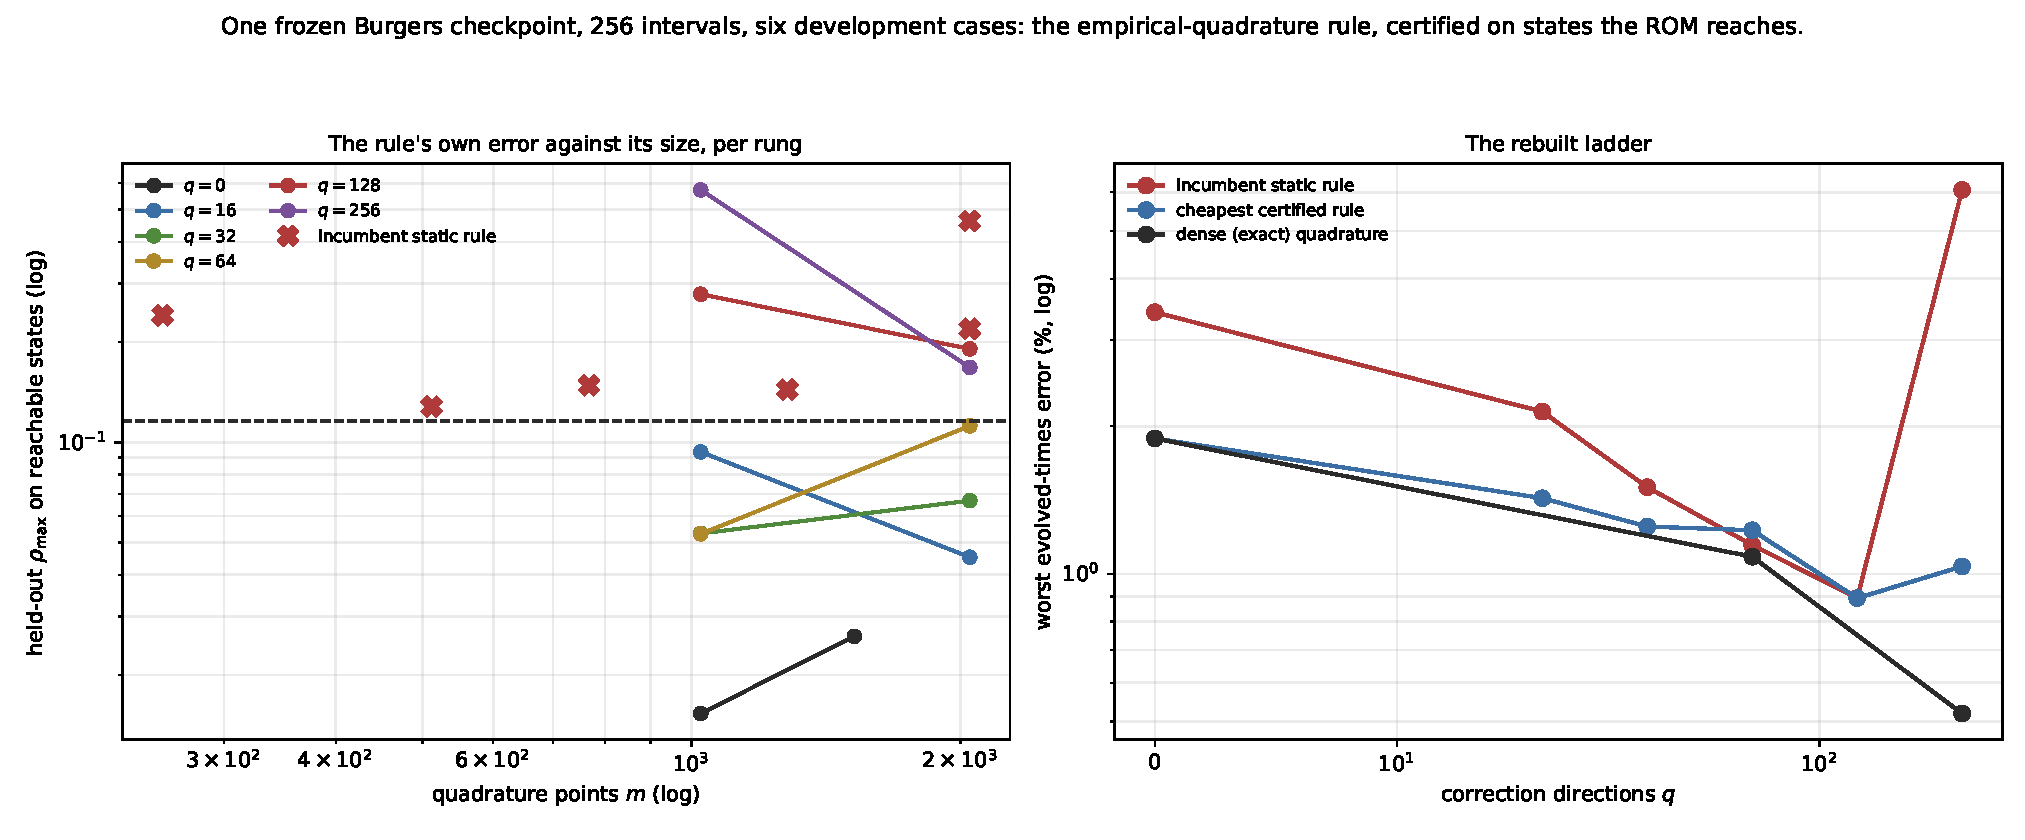
\includegraphics[width=\linewidth]{2026-09-16-q-ridge-certification.pdf}\caption{Left: the rule's held-out $\rho$ against its size $m$, per rung, with the declared bar. Right: the rebuilt ladder against the incumbent rule and the dense twins.}\end{figure}
\begin{figure}[htbp]\centering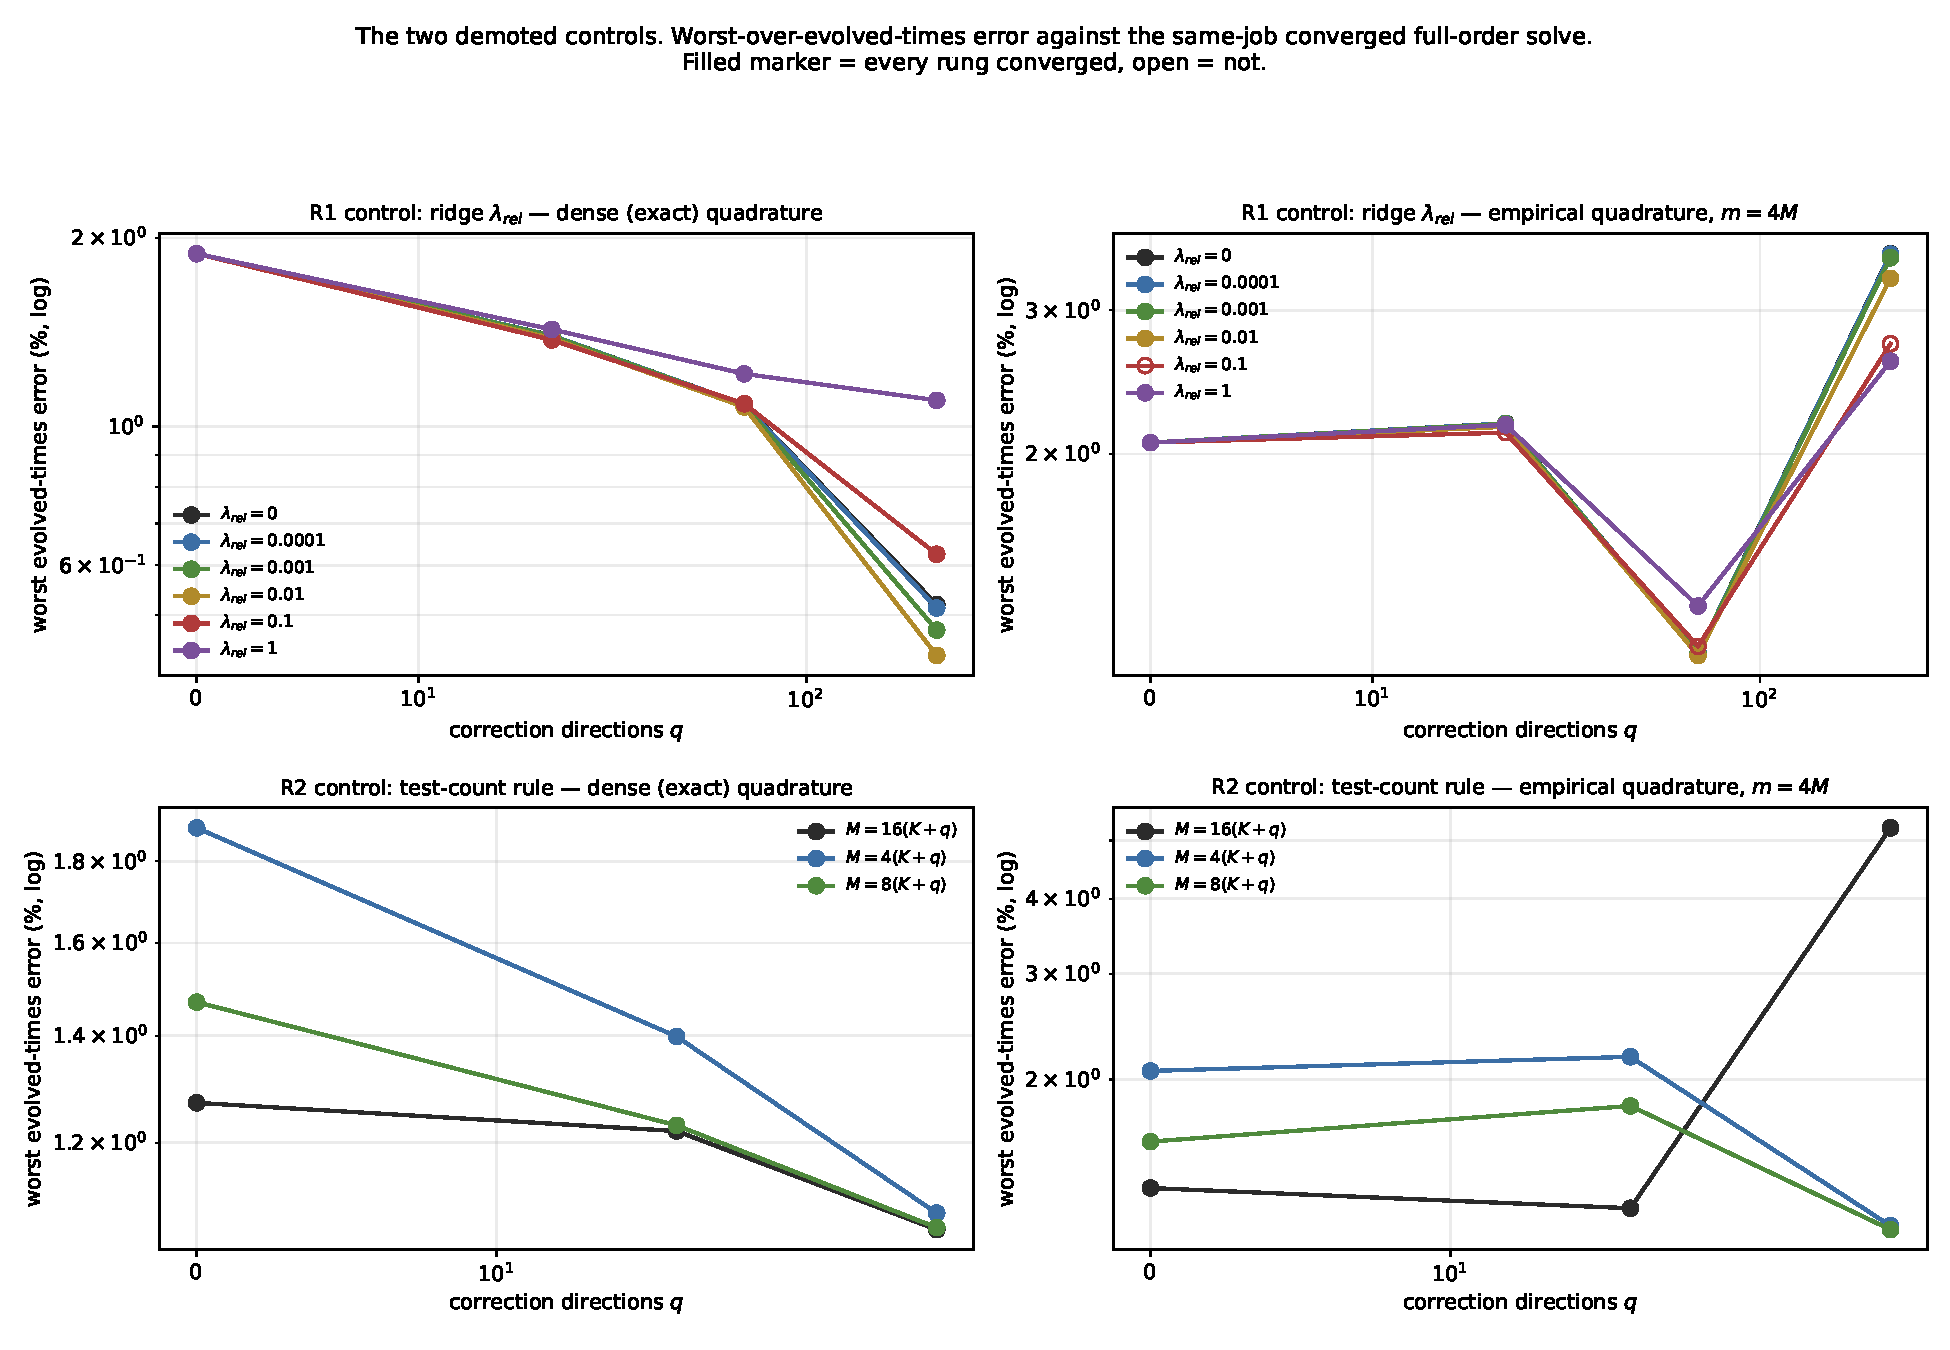
\includegraphics[width=\linewidth]{2026-09-16-q-ridge-controls.pdf}\caption{The two demoted controls: the ridge (top) and the test-count rule (bottom), dense (left) and empirical (right) quadrature.}\end{figure}
\subsection{Glossary}
\begin{itemize}
\item \textbf{$q$} --- the number of extra correction directions added to the frozen neural head. The solved state is $u = G(h_\theta(z) + C_q y)$ with $z \in \mathbb{R}^{16}$ the latent code and $y \in \mathbb{R}^{q}$ the corrections. $q = 0$ is the incumbent reduced-order model.
\item \textbf{rung} --- one value of $q$ in the ladder. "The ladder" is the sequence of rungs at a fixed rule for everything else.
\item \textbf{$M$} --- the number of weak test equations the per-step solve is graded on: $M$ sine modes of the square, in ascending discrete-Laplacian order. The incumbent rule is $M = 4(K+q)$, four tests per unknown.
\item \textbf{$m$} --- the number of grid points the empirical-quadrature rule keeps when it approximates the advection integral. The dense arms use every interior point (65\textbackslash\{\},025 of them) and have no $m$.
\item \textbf{dense / EQ quadrature} --- dense evaluates the advection integral exactly on the grid; EQ replaces it with a nonnegative $m$-point rule fitted offline. Same unknowns, same tests, different integral.
\item \textbf{$\rho$} --- the rule's own relative error on the advection functional it is the only approximation of: $\rho(u) = \|\sum_j w_j \Phi(x_j) a(u)(x_j) - \Phi^\top a(u)\| / \|\Phi^\top a(u)\|$. It is a property of a rule and a state, not of a solve.
\item \textbf{$\rho^\star$, the bar} --- the value a rule's worst held-out $\rho$ must not exceed to be certified. Declared before the job ran at 0.116, the value the q-diag lane measured for the $q=0$ incumbent rule at the state that carries the whole first-interval penalty.
\item \textbf{reachable states} --- states the reduced model actually visits: every Levenberg-Marquardt iterate of its own dense-quadrature rollouts on training-family trajectories. The incumbent rule is instead fitted on static decoder outputs, which is the difference this lane isolates.
\item \textbf{held-out (rules)} --- the certification states come from training-family trajectories disjoint from the ones the rule was fitted on, and both are disjoint from the six evaluation cases.
\item \textbf{held-out test modes} --- sine modes the solve never saw, used only afterwards to measure the weak residual. If a solve were overfitting its $M$ tests, the residual on these would rise with $q$.
\item \textbf{in-space residual} --- the same weak residual on the arm's own $M$ modes, integrated exactly. For a converged dense arm it is essentially zero; for an EQ arm it is not, because the solve drove the quadrature-approximated residual to zero instead.
\item \textbf{per-mode RMS} --- a residual norm divided by the square root of the number of modes, so blocks of different size are comparable; normalised again by the per-node RMS of the previous state to make it dimensionless.
\item \textbf{$\lambda_{rel}$} --- the dimensionless ridge strength of the demoted R1 control. The solve minimises $\|r_w\|^2 + \lambda\|y\|_W^2$ with $W$ the field metric and $\lambda = \lambda_{rel}\sigma_q^2$; $\lambda_{rel} = 0$ is the incumbent solve exactly.
\item \textbf{$\sigma_q$} --- the largest singular value of $\Phi^\top G C_q$, the exact linear response of the weak residual to the corrections. It is what makes $\lambda_{rel}$ dimensionless and comparable across $q$, $M$ and quadrature.
\item \textbf{worst all-times error} --- the largest relative error over the six output times, the six cases included; $t=0$ is included, where the error is the decoder's compression of the supplied initial field.
\item \textbf{worst evolved-times error} --- the same quantity over $t>0$ only -- the trajectory error proper, with the compression term removed.
\item \textbf{$t=0$ compression} --- the relative error at $t=0$: how well the reduced model can represent the initial field it was handed. It uses no quadrature at all, which is why every arm at a given $q$ agrees there.
\item \textbf{same-grid metric} --- error measured against the same job's own converged full-order solve (fft\_tight) on the same 256-interval grid, so the discretisation error cancels.
\item \textbf{converged} --- every one of the 900 solved steps exited on the gradient, residual or tiny-step criterion -- no step ran out of its 600-iteration budget -- and the worst normalised joint gradient is at or inside $10^{-6}$.
\item \textbf{budget exit} --- a time step that stopped because it hit the iteration budget rather than a convergence criterion. Any budget exit disqualifies a rung.
\item \textbf{NNLS relative fit} --- the residual of the nonnegative least-squares problem the rule is fitted by. It is reported but never used to certify a rule: it is flat across rules whose $\rho$ differs by an order of magnitude.
\item \textbf{truncated} --- the fitter ran out of its declared walltime before reaching the target $m$. A truncated rule is disqualified.
\item \textbf{fft\_tight / fft\_loose / nt1e-2\_dt01} --- same-job full-order Newton solves at three tolerance/time-step settings. fft\_tight is the reference the same-grid metric is measured against, so its own error is zero by construction.
\item \textbf{cross-job fidelity} --- a named arm of this lane reproducing a named arm of an earlier audited job to a declared tolerance. It is how the lane proves it changed only what it said it changed.
\end{itemize}
\end{document}
